\documentclass[11pt]{article}
\usepackage[a4paper, margin=2.3cm]{geometry}
\usepackage[T1]{fontenc}
\usepackage{lmodern}
\usepackage{microtype}
\usepackage{graphicx}
\usepackage{float}
\usepackage{amsmath, amssymb}
\usepackage{xcolor}
\usepackage{booktabs}
\usepackage{array}
\usepackage{enumitem}
\usepackage{fancyhdr}
\usepackage{titlesec}
\usepackage[most]{tcolorbox}
\usepackage[font=small, labelfont=bf]{caption}
\usepackage[colorlinks=true, linkcolor=navy, urlcolor=navy]{hyperref}

% ---------- colours ----------
\definecolor{navy}{HTML}{1F3A5F}
\definecolor{teal}{HTML}{1B7F79}
\definecolor{amber}{HTML}{C77D0A}
\definecolor{brick}{HTML}{B03A2E}
\definecolor{leaf}{HTML}{2E7D32}
\definecolor{paper}{HTML}{F6F7F9}

% ---------- layout ----------
\setlength{\parskip}{0.55em}
\setlength{\parindent}{0pt}
\renewcommand{\arraystretch}{1.25}
\setlist{itemsep=0.2em, topsep=0.3em}
\pagestyle{fancy}
\fancyhf{}
\fancyhead[L]{\small\textcolor{navy}{Lab 7 -- MBIST on dtmf\_recvr\_core}}
\fancyhead[R]{\small R Sarang -- EC23I2015}
\fancyfoot[C]{\small\thepage}
\renewcommand{\headrulewidth}{0.4pt}
\titleformat{\section}{\Large\bfseries\color{navy}}{\thesection}{0.6em}{}
\titleformat{\subsection}{\large\bfseries\color{teal}}{\thesubsection}{0.6em}{}
\titleformat{\subsubsection}{\normalsize\bfseries\color{navy}}{\thesubsubsection}{0.6em}{}
\newcommand{\code}[1]{\texttt{\small #1}}

% ---------- call-out boxes ----------
\newtcolorbox{whybox}[1][Why are we doing this?]{
  enhanced, breakable, colback=teal!7, colframe=teal, fonttitle=\bfseries,
  title={#1}, boxrule=0.6pt, arc=2pt, left=6pt, right=6pt, top=4pt, bottom=4pt}
\newtcolorbox{keybox}[1][Key idea]{
  enhanced, breakable, colback=amber!8, colframe=amber, fonttitle=\bfseries,
  title={#1}, boxrule=0.6pt, arc=2pt, left=6pt, right=6pt, top=4pt, bottom=4pt}
\newtcolorbox{resultbox}[1][Result]{
  enhanced, breakable, colback=leaf!8, colframe=leaf, fonttitle=\bfseries,
  title={#1}, boxrule=0.6pt, arc=2pt, left=6pt, right=6pt, top=4pt, bottom=4pt}
\newtcolorbox{probbox}[1][The problem]{
  enhanced, breakable, colback=brick!7, colframe=brick, fonttitle=\bfseries,
  title={#1}, boxrule=0.6pt, arc=2pt, left=6pt, right=6pt, top=4pt, bottom=4pt}

% \shot{file}{width-fraction}{caption}
\newcommand{\shot}[3]{%
  \begin{figure}[H]\centering
  \includegraphics[width=#2\textwidth]{images/#1}
  \caption{#3}
  \end{figure}}

\title{\vspace{-1em}\textbf{\color{navy}Lab 7: Memory BIST on \code{dtmf\_recvr\_core}}\\[2pt]
\large Insertion, Controller Reconfiguration, SMarch Algorithm and Fault Detection}
\author{\textbf{R Sarang}\quad|\quad Roll No: EC23I2015\\
        EC5034 -- VLSI Testing Practice}
\date{\today}

\begin{document}
\maketitle
\vspace{-1.2em}

\begin{tcolorbox}[enhanced, colback=paper, colframe=navy!40, boxrule=0.5pt, arc=2pt]
\textbf{Report at a glance}
\begin{itemize}[leftmargin=1.4em, itemsep=1pt]
  \item \textbf{Goal:} insert Memory BIST into the DTMF receiver core (5 memories), then change the BIST
        configuration (new controller, sequential steps, SMarch algorithm) and prove that the BIST detects an injected memory fault.
  \item \textbf{Tools:} Siemens Tessent Shell 2022.4 (insertion) $\rightarrow$ QuestaSim (simulation)
        $\rightarrow$ Cadence Genus (synthesis) and Conformal (LEC).
  \item \textbf{Headline results:} all tasks simulate with \textbf{pass 3, fail 0}; pre-MBIST vs post-MBIST RTL LEC
        \textbf{573 points, 0 non-equivalent}; Stage 2A and 2B LEC \textbf{PASS}; the injected fault gives
        \textbf{2 miscompares} and drives the c4 \code{MBISTPG\_GO} low.
  \item \textbf{Area cost of MBIST:} cell area only \textbf{+2.38\%} (memories dominate), total power \textbf{+6.35\%}.
\end{itemize}
\end{tcolorbox}

\tableofcontents
\newpage

% =====================================================================
\section{Introduction and Objectives}

Memory BIST (MBIST) places a small test controller on the chip that writes and reads March-style patterns into every
embedded memory and reports a pass/fail verdict (\code{MBISTPG\_GO}, \code{MBISTPG\_DONE}). Lab 6 inserted it into a
simple counter design. In Lab 7 the same flow is applied to a larger design, \code{dtmf\_recvr\_core}, which has
\textbf{five memories on three different clocks}, and the BIST configuration is then changed in three ways.

\begin{center}
\small
\begin{tabular}{@{}cp{4.1cm}p{8.4cm}@{}}
\toprule
\textbf{Task} & \textbf{Title} & \textbf{What is done} \\ \midrule
1 & MBIST insertion & Clocks, DRC, DFT specification, ROM preload, insertion, signoff simulation, pre/post-MBIST LEC, synthesis, two-stage LEC \\
2 & Controller change & New controller \code{c4}; memories \code{\_2} and \code{\_3} moved to it and tested \emph{in parallel} \\
3 & Algorithm change & Two sequential steps in \code{c4}; step 2 runs \code{SMarch}; full address range (\code{reduced\_address\_count off}) \\
4 & Fault injection & One RAM location is corrupted between W0 and R0; the BIST must flag it \\ \bottomrule
\end{tabular}
\end{center}

\begin{whybox}[Working style and change log]
Every edit that goes beyond a path or file-name fix was logged with what, where and why in \code{lab7\_changes\_log.md}.
The main changes are quoted in the relevant sections below.
\end{whybox}

% =====================================================================
\section{Design Under Test}

\code{dtmf\_recvr\_core} is a DTMF receiver (power manager, PLL, test-control block, TDSP core, SPI, DMA, arbiter, etc.).
Five memories are compiled. All RAMs wrap the same \code{ram\_256x16A} model; the 128-word RAM pads its address
with a constant \code{1'b0}.

\begin{center}
\small
\begin{tabular}{@{}llll@{}}
\toprule
\textbf{Memory instance} & \textbf{Type} & \textbf{Clock net} & \textbf{Note} \\ \midrule
\code{RAM\_128x16\_TEST\_INST} & RAM 128$\times$16 & \code{m\_ram\_clk} & \\
\code{RAM\_256x16\_TEST\_INST\_1} & RAM 256$\times$16 & \code{m\_dsram\_clk} & original data-sample RAM \\
\code{RAM\_256x16\_TEST\_INST\_2} & RAM 256$\times$16 & \code{m\_dsram\_clk} & new in Lab 7 \\
\code{RAM\_256x16\_TEST\_INST\_3} & RAM 256$\times$16 & \code{m\_dsram\_clk} & new in Lab 7 \\
\code{ROM\_512x16\_0\_INST} & ROM 512$\times$16 & \code{m\_clk} & needs a preload file \\ \bottomrule
\end{tabular}
\end{center}

\begin{keybox}[Q1: the two new memory instances]
In Lab 6's RTL there was a single \code{RAM\_256x16\_TEST\_INST}. In \code{dtmf\_recvr\_core.v} that instance now sits inside an
\code{`ifdef orig} (not compiled) and is replaced by three \emph{chained} instances: \code{RAM\_256x16\_TEST\_INST\_1}
(\code{dout} feeds \code{din} of \code{\_2}), \code{\_2} (feeds \code{\_3}) and \code{\_3} (drives \code{ds\_data}).
The two new instances are therefore \textbf{\code{RAM\_256x16\_TEST\_INST\_2}} and \textbf{\code{RAM\_256x16\_TEST\_INST\_3}}.
\end{keybox}

% =====================================================================
\section{Task 1: Memory BIST Insertion}

\subsection{Tessent set-up, clocks and DRC}

The flow follows Lab 6's \code{run\_mbist\_insertion} script, typed into Tessent one line at a time. Only the design name
changed (\code{processor\_core} $\rightarrow$ \code{dtmf\_recvr\_core}). A new \code{rtl\_file\_list} was created with
\code{timescale.h} first and the 27 RTL files after it.

\shot{task1_step04_tessent_shell_start.png}{0.9}{Step 4: Tessent Shell 2022.4 started from \code{dtmf\_recvr/mbist} with a log file; the prompt is \code{SETUP>}. The first lines of the script (\code{set\_context dft -rtl}, TSDB directory, cell library, memory models, RTL) are run from here.}

After the primary clock \code{add\_clocks 0 refclk -period 8.0ns -label refclk}, the first \code{check\_design\_rules} produces the
expected \textbf{DFT\_C1 violation}.

\shot{task1_step07_drc_c1_violation.png}{0.9}{Step 7: DRC violation \code{DFT\_C1}. Source tracing of the memory clock pin \code{RAM\_128x16\_TEST\_INST/RAM\_128x16\_INST/CLK} stops at \code{TEST\_CONTROL\_INST/rtlc0\_7/muxinst/Z}, because Tessent does not know how the memory clocks are derived from \code{refclk}.}

\begin{keybox}[Q2: ROM clock path and the reason for DFT\_C1]
Tracing backwards from the ROM: \code{ROM\_512x16\_0\_INST/CLK} $\leftarrow$ net \code{m\_clk} $\leftarrow$ multiplexer
\code{rtlc0\_7/muxinst} in \code{TEST\_CONTROL\_INST} (\code{assign m\_clk = test\_mode ? scan\_clk : clk;}) $\leftarrow$ net \code{clk}
$\leftarrow$ \code{PLLCLK\_INST/clk2x} $\leftarrow$ primary input \code{refclk}. The tracing cannot pass the multiplexer: \code{test\_mode} is
unknown and \code{clk} (a PLL output) has no declared relation to \code{refclk}.
\end{keybox}

\begin{figure}[H]\centering
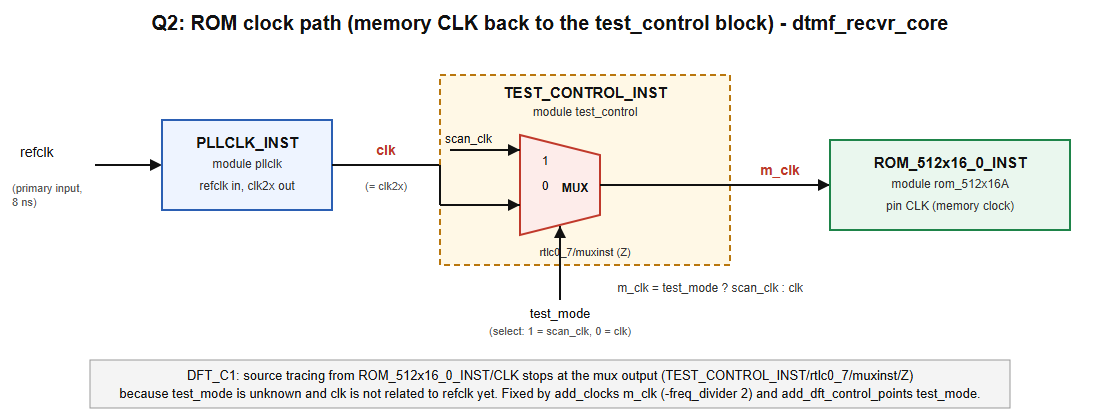
\includegraphics[width=0.97\textwidth]{images/q2_rom_clock_path.png}
\caption{Q2 diagram: ROM clock generation from the memory clock pin back to the test-control block. The multiplexer selects \code{scan\_clk} in test mode and \code{clk} in mission mode.}
\end{figure}

The fix is to describe the derived clocks (divider 2 gives 16\,ns from 8\,ns), name the \code{test\_mode} signal and create a control point for it:

\begin{center}\small\ttfamily
\begin{tabular}{@{}l@{}}
add\_clocks TEST\_CONTROL\_INST/m\_clk -reference refclk -label m\_clk -freq\_divider 2\\
add\_clocks TEST\_CONTROL\_INST/m\_ram\_clk -reference refclk -label m\_ram\_clk -freq\_divider 2\\
add\_clocks TEST\_CONTROL\_INST/m\_dsram\_clk -reference refclk -label m\_dsram\_clk -freq\_divider 2\\
register\_static\_dft\_signal\_names test\_mode\\
add\_dft\_control\_points TEST\_CONTROL\_INST/test\_mode -dft\_signal\_source\_name test\_mode
\end{tabular}
\end{center}

\shot{task1_step08_clocks_and_drc_clean.png}{0.9}{Step 8: derived clocks added (warning about the pseudo primary input is expected). The \code{test\_mode} control point is created with a TDR bit, and the re-run of \code{check\_design\_rules} no longer reports DFT\_C1; the prompt moves from \code{SETUP>} to \code{ANALYSIS>}.}

\subsection{Memory report and DFT specification}

\shot{task1_step09_report_memory_instances.png}{0.9}{Step 9: \code{report\_memory\_instances}. Five memories are found, with the clocks listed in Section~2.}

\begin{keybox}[Q3: how many memories?]
\textbf{Five}, matching the five compiled instances of \code{dtmf\_recvr\_core.v}: the 128$\times$16 RAM, three 256$\times$16 RAMs and the
512$\times$16 ROM. The sixth, original \code{RAM\_256x16\_TEST\_INST}, is inside \code{`ifdef orig} and is not compiled, so it is
correctly absent. Instance paths and clocks agree with the RTL.
\end{keybox}

\shot{task1_step10_dft_specification.png}{0.9}{Step 10: \code{create\_dft\_specification} and \code{report\_config\_data}. The generated plan contains three controllers; the ROM interface still has the placeholder \code{<path\_to\_rom\_content\_file>}.}

\begin{keybox}[Q4: controllers and memory interfaces]
\begin{center}\small
\begin{tabular}{@{}llll@{}}
\toprule
\textbf{Controller} & \textbf{Clock label} & \textbf{Interface} & \textbf{Memory instance} \\ \midrule
c1 & \code{m\_ram\_clk} & m1 & \code{RAM\_128x16\_TEST\_INST/RAM\_128x16\_INST} \\
c2 & \code{m\_dsram\_clk} & m1 & \code{RAM\_256x16\_TEST\_INST\_1/RAM\_256x16\_INST} \\
 & & m2 (reused m1) & \code{RAM\_256x16\_TEST\_INST\_2/RAM\_256x16\_INST} \\
 & & m3 (reused m1) & \code{RAM\_256x16\_TEST\_INST\_3/RAM\_256x16\_INST} \\
c3 & \code{m\_clk} & m1 & \code{ROM\_512x16\_0\_INST} \\ \bottomrule
\end{tabular}
\end{center}
\end{keybox}

\subsection{ROM preload and insertion}

\code{process\_dft\_specification} first failed because the ROM content file was undefined. A 512-line file \code{romcontent.cfg}
(random 4-digit hexadecimal values, one per line, 16-bit width) was created and attached to controller \code{c3} in the
\code{display\_specification} GUI (shown in Figure~\ref{fig:romgui} of Task~2, which uses the same GUI session). The
configuration was validated and exported as \code{mbistTask1.cfg}, then read back with \code{read\_config\_data} and processed.
Insertion created the IJTAG SIBs, the TDR, controllers \code{c1}--\code{c3} and the BIST access port. ICL was extracted and the
Genus import script written.

\subsection{Signoff simulation}

Patterns were created and simulated (\code{ICLNetwork}, \code{MemoryBist\_P1}, \code{MemoryBist\_ParallelRetentionTest\_P1}).
The first run \textbf{failed} \code{MemoryBist\_P1} with 25 miscompares. The simulation log showed
\code{Failed to open readmem file romcontent.hex}: Tessent copies the preload file as \code{romcontent.cfg}, but the model
\code{rom\_512x16A.v} reads \code{romcontent.hex}. Changing the \code{\$readmemh} argument to \code{romcontent.cfg} (change \#5 in the log)
fixed it.

\shot{task1_step18_simulations_fail_then_pass3.png}{0.9}{Step 18: first run \textbf{pass 2, fail 1} (ROM read as \code{xxxx}); after the \code{\$readmemh} file-name fix, the re-run gives \textbf{pass 3, fail 0}.}

\subsection{Waveform snapshots (\code{MemoryBist\_P1})}

\shot{task1_step18_wave_controllers_en_go_done.png}{0.95}{Controller signals \code{MBISTPG\_EN}, \code{MBISTPG\_GO}, \code{MBISTPG\_DONE} for c1, c2 and c3. The RAM controllers c1 and c2 finish at about 38--42\,$\mu$s; the ROM controller c3 finishes at about 67--68\,$\mu$s (512 words).}

\shot{task1_step18_wave_controllers_with_collar_en.png}{0.95}{Same waveform with \code{BIST\_COLLAR\_EN*} added. c2 has three collar enables (one per memory, EN0/EN1/EN2), c1 and c3 only EN0. The RAM enables pulse at about 30--38\,$\mu$s; c3's EN0 stays high from about 30 to 68\,$\mu$s.}

\shot{task1_step18_wave_memories_addr_data_ctrl.png}{0.95}{Memory address, data and control (\code{Q, CLK, CEN, WEN, A, D}) of all five memories. The RAMs are active inside their controller windows; the ROM shows an address sweep with no \code{WEN} or \code{D} pins.}

\subsection{Pre-MBIST vs post-MBIST RTL LEC}

The Lab 6 \code{mbist.do} was adapted (memory models, 5 BIST-select constraints, \code{pllclk} source, \code{test\_mode} constrained to 0 in both designs;
changes \#6--\#9 in the log) and run as \code{lec -XL -nogui -dofile mbist.do}.

\shot{task1_step19_prembist_postmbist_lec_pass.png}{0.8}{Pre-MBIST vs post-MBIST RTL equivalence: \textbf{573 compared points, all equivalent} (36 PO, 533 DFF, 4 BBOX), 0 non-equivalent. The extra registers in the revised design are MBIST-only logic.}

\begin{resultbox}[Why the first attempts failed]
(1)~A library path from Lab 6 did not exist on this server (path fix). (2)~\code{pllclk} was undefined; it is read from \code{library/memories}.
(3)~With \code{test\_mode} unconstrained there were 536 non-equivalent points, all behind the clock multiplexers. In the inserted design
\code{test\_mode} is multiplexed with IJTAG bits, so pinning \code{test\_mode} and the multiplexer output to 0 puts both designs in mission mode.
\end{resultbox}

\subsection{Synthesis and the two-stage LEC}

Genus ran \code{syn\_generic}, \code{syn\_map} and \code{syn\_opt} with \code{constraints.sdc}, and wrote the netlist, reports and the LEC
scripts (\code{rtl2fvmap.tcl}, \code{fvmap2final.tcl}). For the comparison, the \emph{pre-MBIST} design was synthesised too (\code{synth\_prembist}, same libraries and constraints).

\shot{task1_step20_prembist_qor_power.png}{0.9}{Genus QoR and power for the \textbf{pre-MBIST} design.}
\shot{task1_step20_postmbist_qor_power.png}{0.9}{Genus QoR and power for the \textbf{post-MBIST} design.}

\begin{center}
\small
\begin{tabular}{@{}lrrr@{}}
\toprule
\textbf{Metric} & \textbf{Pre-MBIST} & \textbf{Post-MBIST} & \textbf{Change} \\ \midrule
Leaf instances & 6074 & 9678 & +3604 (+59.3\%) \\
Sequential instances & 515 & 1113 & +598 (+116\%) \\
Combinational instances & 5559 & 8565 & +3006 (+54.1\%) \\
Hierarchical instances & 1 & 45 & +44 \\
Cell area & 285606.583 & 292396.909 & +6790.3 (+2.38\%) \\
Total power (vectorless) & 1.81259e-02 W & 1.92764e-02 W & +1.15 mW (+6.35\%) \\
\code{m\_clk} slack & 0.0 ps & 0.7 ps & no violation \\
Other clock slacks (digit/dsram/ram/rcc/spi, ps) & 7466/3360/3857/2213/14408 & 7466/2575/3428/2607/14604 & no violation \\
Extra timing groups & none & tessent\_tck, bap1\_tck, bap1\_interfaces\_tck & no violation \\ \bottomrule
\end{tabular}
\end{center}

\begin{keybox}[Reading the comparison]
Instances rise by almost 60\% but area only by 2.4\%, because the five memories (black boxes) dominate the area. Memory power share falls
from 31.7\% to 11.4\% while clock power rises from 6.8\% to 26.2\% (new \code{tessent\_tck}/BAP clocks). All timing groups still meet timing.
\end{keybox}

Stage 2A compares the post-MBIST RTL with Genus's \code{fv\_map}: first pass 529 equivalent and 51 aborted flip-flops, then, after
\code{analyze abort -compare}, \textbf{580 compared points all equivalent, 0 abort, 0 non-equivalent}. Stage 2B compares \code{fv\_map} with
the final netlist: \textbf{LEC Comparison PASS, Flatten Comparison PASS}.

\shot{task1_step20_lec_stage2b_pass.png}{0.9}{Stage 2B LEC (\code{fv\_map} vs final netlist \code{dtmf\_recvr\_core.vg}): both comparisons PASS.}

% =====================================================================
\section{Task 2: Adding a Controller (Parallel Test)}

\textbf{Goal:} move memories \code{\_2} and \code{\_3} from controller c2 to a new controller c4 so that both are tested \emph{in parallel}.
A separate working directory \code{mbist\_task2} (with its own \code{tsdb\_outdir}) keeps Task 1's results intact.

\subsection{Setup in the new directory}

\shot{task2_step03_tessent_shell_start_set_context.png}{0.75}{Tessent restarted in \code{mbist\_task2} with its own log; \code{set\_context dft -rtl -design\_id rtl1} is entered.}
\shot{task2_step03_tsdb_and_cell_library.png}{0.7}{New TSDB output directory and cell library are read, so Task 1's \code{tsdb\_outdir} is not overwritten.}
\shot{task2_step03_clocks_pport_warning.png}{0.7}{Derived clocks re-added; the pseudo primary-input warning is expected (same as in Task 1).}

\subsection{Editing the configuration in the GUI}

The same setup as Task 1 was run up to \code{create\_dft\_specification}, then \code{read\_config\_data mbistTask1.cfg} (keeps the ROM file), and
\code{display\_specification} opened the editor.

\begin{figure}[H]\centering
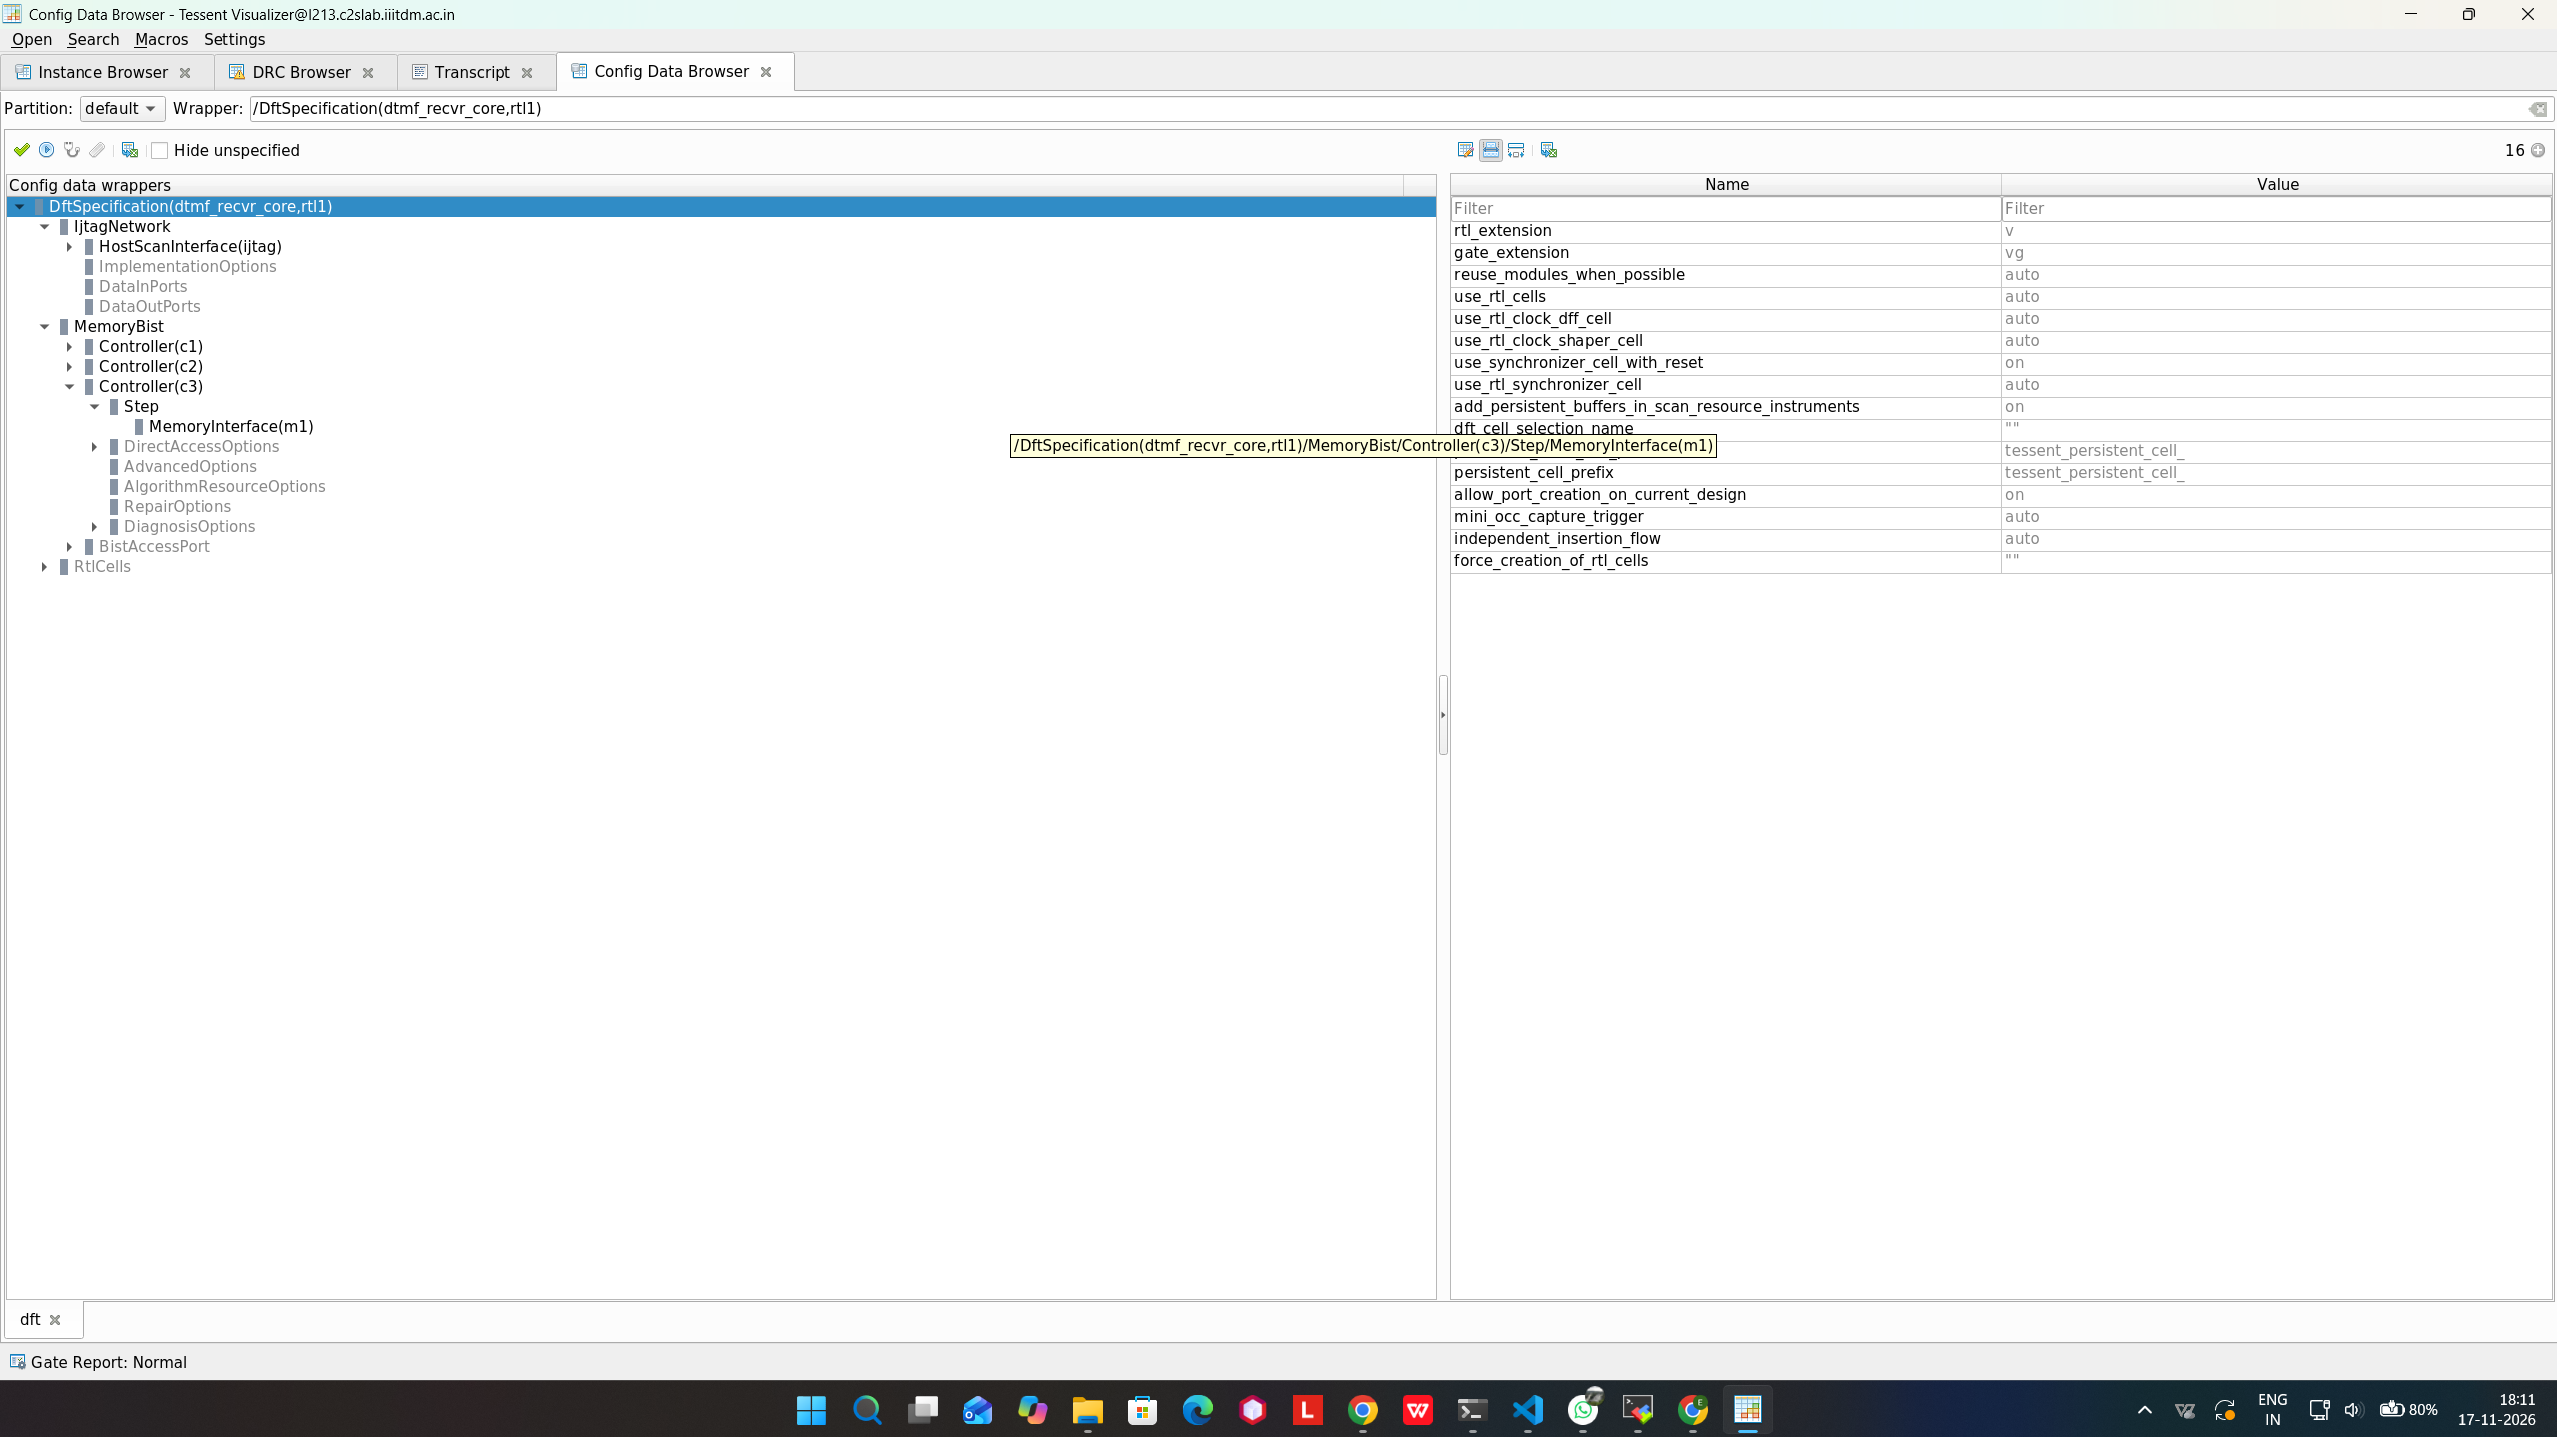
\includegraphics[width=0.9\textwidth]{images/task2_step04_gui_opened_config_browser.png}
\caption{\code{display\_specification}: configuration browser with the wrapper tree on the left and properties on the right.}
\end{figure}
\begin{figure}[H]\centering
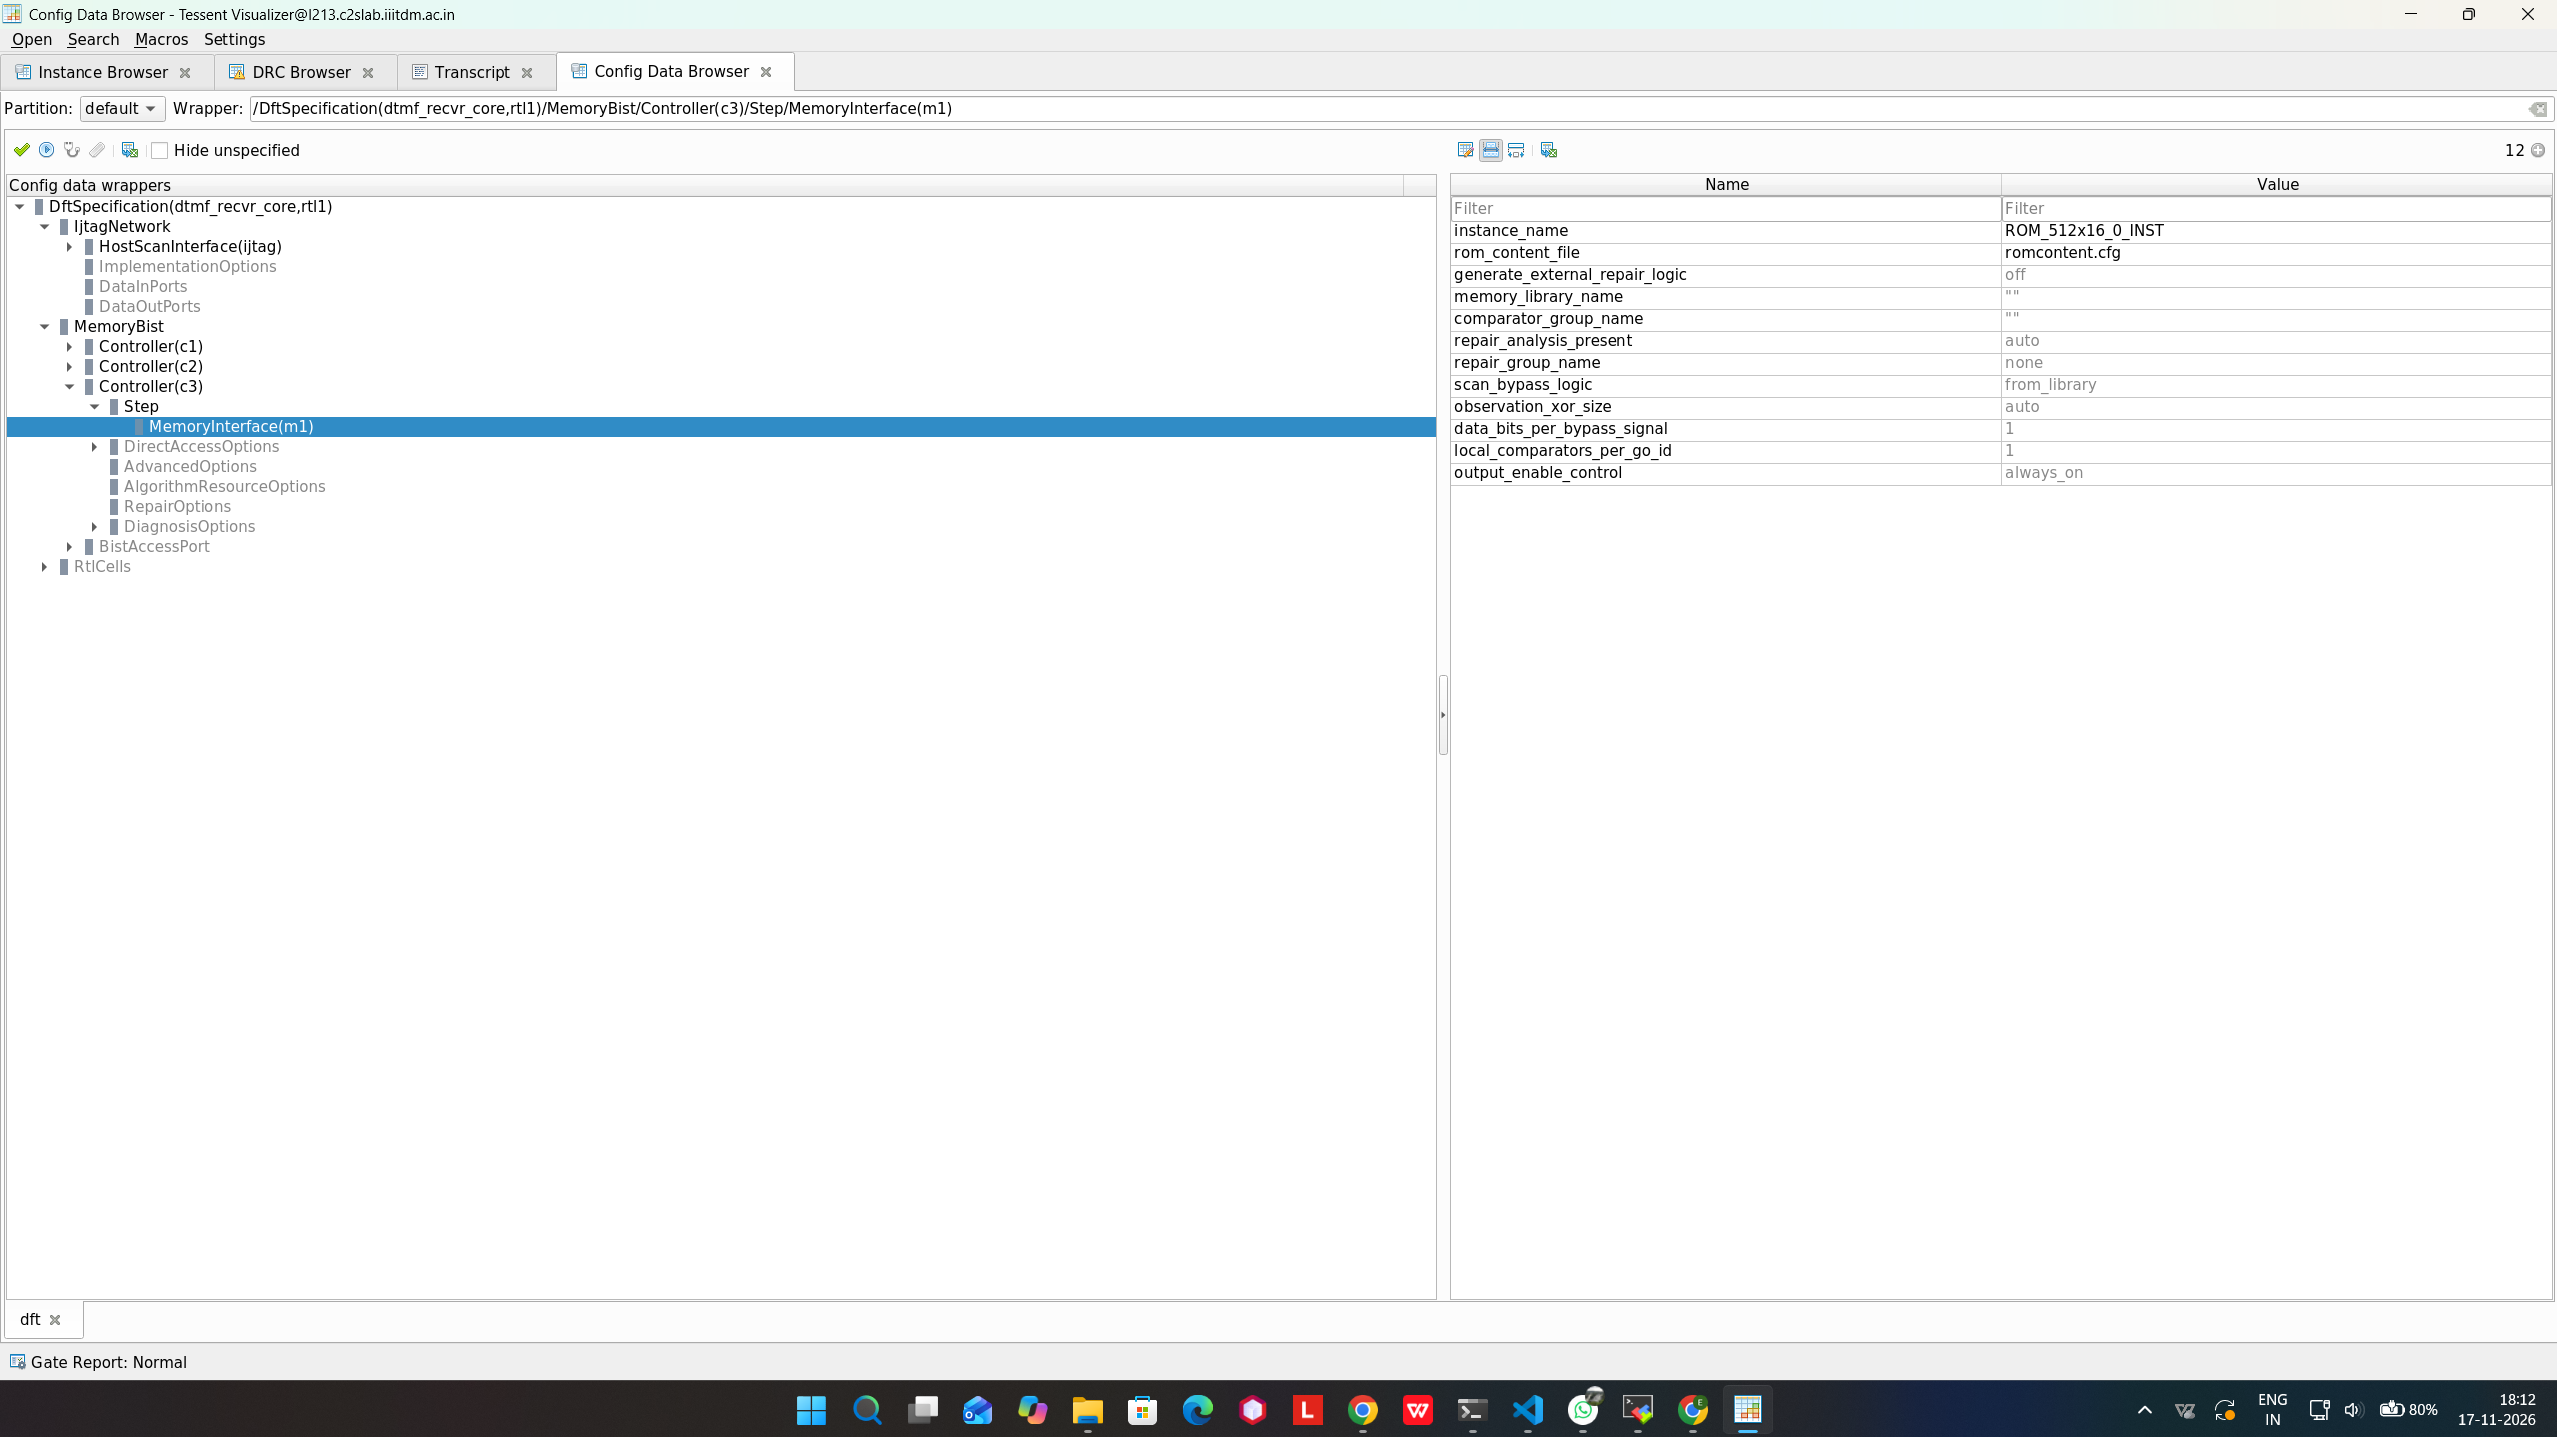
\includegraphics[width=0.9\textwidth]{images/task2_step04_gui_rom_content_loaded.png}
\caption{Controller c3 / Step / MemoryInterface m1: \code{rom\_content\_file = romcontent.cfg} is set (carried from Task 1).\label{fig:romgui}}
\end{figure}

\shot{task2_step04_controller_c4_added.png}{0.9}{Step 3: \textbf{Add wrapper as child} on \code{MemoryBist}; wrapper \code{Controller} with id \code{c4}.}
\shot{task2_step04a_c2_clock_domain_label.png}{0.9}{Step 4a: controller c2's \code{clock\_domain\_label} is \code{m\_dsram\_clk}.}
\shot{task2_step04b_c4_clock_domain_label.png}{0.9}{Step 4b: the same clock label is set on c4, since the moved memories are clocked by \code{m\_dsram\_clk}.}
\shot{task2_step04c_c4_step_added.png}{0.9}{Step 4c: a \code{Step} wrapper added under c4.}
\shot{task2_step04d_c2_m2_instance_name.png}{0.9}{Step 4d: instance path of c2's interface m2 noted (\code{RAM\_256x16\_TEST\_INST\_2/RAM\_256x16\_INST}).}
\shot{task2_step04d_c2_m3_instance_name.png}{0.9}{Step 4d: instance path of c2's interface m3 noted (\code{RAM\_256x16\_TEST\_INST\_3/RAM\_256x16\_INST}).}
\shot{task2_step04e_c4_m1_added.png}{0.9}{Step 4e: \code{MemoryInterface} m1 added under the c4 Step.}
\shot{task2_step04f_c4_m2_added.png}{0.9}{Step 4f: second \code{MemoryInterface} m2 added under the same c4 Step (both in one step means parallel test).}
\shot{task2_step04g_c4_m1_instance_name.png}{0.9}{Step 4g: c4/m1 \code{instance} set to \code{RAM\_256x16\_TEST\_INST\_2/RAM\_256x16\_INST}.}
\shot{task2_step04h_c4_m2_instance_name.png}{0.9}{Step 4h: c4/m2 \code{instance} set to \code{RAM\_256x16\_TEST\_INST\_3/RAM\_256x16\_INST}.}
\shot{task2_step04i_c2_reused_interfaces_deleted.png}{0.9}{Steps 4i--4j: the two \code{ReusedMemoryInterface} entries m2 and m3 deleted from c2, which now keeps only m1 (\code{\_1}).}

\begin{keybox}[Note on the lab text]
The handout says to delete m2 from c2 and m3 from c3. In this design c3 only has the ROM (m1); both reused interfaces m2 and m3 belong to
\textbf{c2}, so both were deleted from c2 (change \#12 in the log).
\end{keybox}

\shot{task2_step04k_save_mbist_task2_cfg_dialog.png}{0.7}{Step 4k: after validation (green tick, only an expected warning that \code{\_2}/\code{\_3} will be uniquified because they no longer reuse c2's interface), the configuration is exported as \code{mbist\_task2.cfg}.}

\subsection{Insertion and simulation}

\code{read\_config\_data mbist\_task2.cfg}, \code{process\_dft\_specification} (now four controllers c1--c4), ICL extraction, pattern generation and simulation
were repeated as in Task 1.

\shot{task2_step18_simulations_pass3.png}{0.8}{Task 2 simulation result: \textbf{pass 3, fail 0}.}
\shot{task2_step05_vsim_hierarchy.png}{0.45}{Questa structure view: the c4 controller instance sits directly under \code{DUT\_inst}, next to c3; its signals are added to the waveform.}

\subsection{Waveform review}

\shot{task2_step18_wave_c4_controller_signals_first_view.png}{0.95}{First view of c4: \code{MBISTPG\_EN}, \code{GO}, \code{DONE}, \code{BIST\_COLLAR\_EN0} and \code{EN1}.}
\shot{task2_step18_wave_c4_controller_signals.png}{0.95}{c4 controller signals. \code{BIST\_COLLAR\_EN0} and \code{EN1} rise and fall together (about 43.2 to 46.6\,$\mu$s); \code{GO} rises at about 43\,$\mu$s and \code{DONE} pulses after the collar window.}
\shot{task2_step18_wave_c4_memories_parallel.png}{0.95}{\code{Q, CLK, CEN, WEN, A, D} of \code{RAM\_256x16\_TEST\_INST\_2} and \code{\_3}: the activity is identical in both memories.}
\shot{task2_step18_wave_c4_zoomed_parallel.png}{0.95}{Zoom (42--50\,$\mu$s): \code{WEN}, address, data and \code{Q} of \code{\_2} and \code{\_3} are identical cycle for cycle. \code{xxxx} outside the window is uninitialised memory.}

\begin{resultbox}[Task 2 conclusion]
Both memories under c4 share one step, one collar-enable window and identical pin activity, so they are tested \textbf{in parallel}. The whole c4 test ends at about 47\,$\mu$s.
\end{resultbox}

% =====================================================================
\section{Task 3: SMarch Algorithm and Sequential Test}

\textbf{Goal:} under c4, test \code{\_2} first and \code{\_3} afterwards, with \code{\_3} running the \code{SMarch} algorithm over its full address range.
A new directory \code{mbist\_task3} keeps Task 1 and 2 results.

\shot{task3_step01_gui_task2_config_loaded.png}{0.9}{Task 2's \code{mbist\_task2.cfg} loaded in the GUI as the starting point.}
\shot{task3_step02_c4_second_step_added.png}{0.9}{A second \code{Step} added under c4.}
\shot{task3_step02_m2_moved_to_second_step.png}{0.9}{\code{MemoryInterface} m2 (\code{RAM\_256x16\_TEST\_INST\_3}) cut from the first step and pasted into the second step; m1 stays in step 1. Steps run one after another.}
\shot{task3_step03_algorithm_dialog.png}{0.5}{Editing the \code{algorithm} field of the second step (the default from the TCD memory model is used where it is empty).}
\shot{task3_step03_smarch_set_on_second_step.png}{0.9}{\code{algorithm = SMarch} set on step 2 only.}
\shot{task3_step04_validation_transcript.png}{0.9}{Validation (green tick): only the known uniquify warning.}
\shot{task3_step04_save_mbist_task3_cfg_dialog.png}{0.7}{Configuration exported as \code{mbist\_task3.cfg}.}

\subsection{Complete algorithm run (reduced\_address\_count off)}

By default Tessent simulates a \emph{reduced address set} to save time. For the full algorithm, \code{create\_patterns\_spec} and
\code{report\_config\_data > pattern\_specification.cfg} were run; in that file line 86 (\code{MemoryBist\_P1}) was edited from
\code{reduced\_address\_count : on;} to \code{off;} (change \#15). The retention test was left unchanged. The file was read back, processed and simulated.

\shot{task3_step06_pattern_spec_and_simulations_pass3.png}{0.9}{Grep showing the edited line, pattern processing and the result \textbf{pass 3, fail 0}.}

\subsection{Waveform review}

\shot{task3_step06_wave_c4_sequential_smarch.png}{0.95}{c4 over the whole run: \code{RAM\_256x16\_TEST\_INST\_2} (step 1) is active from about 43 to 224\,$\mu$s with \code{BIST\_COLLAR\_EN0} high; \code{\_3} (step 2, SMarch) is idle until about 224\,$\mu$s and active until about 317\,$\mu$s with \code{EN1} high. \code{GO} stays high; \code{DONE} pulses at the end.}
\shot{task3_step06_wave_w0_sweep_to_r0w1_zoom.png}{0.95}{Zoom on \code{\_3} at the end of the W0 sweep (about 232.6\,$\mu$s) where R0W1 begins. The data pattern on \code{\_3} (0000/ffff/0000/\dots) differs from \code{\_2}.}
\shot{task3_step06_wave_r0w1_address_steps_zoom.png}{0.95}{R0W1 phase of SMarch: two clocks (about 64\,ns) per address, addresses visited in steps of 0x10. This timing is used to choose the fault time in Task 4.}

\begin{resultbox}[Task 3 conclusion]
The two memories under c4 are tested one after another (about 357\,$\mu$s in total versus about 117\,$\mu$s for the parallel Task 2), and step 2 shows the SMarch read/write sequence.
\end{resultbox}

% =====================================================================
\section{Task 4: Fault Injection and Detection}

\subsection{Choosing the fault}

SMarch performs sequences such as W0, R0W1, R1W1, R1W0, R0W0. If a location is corrupted after W0 and before the following R0,
the R0 of that location must read the wrong value. From the Task 3 waveform (\code{RAM\_256x16\_TEST\_INST\_3}):
the clock period is about 32\,ns, R0W1 starts at about 232\,630\,ns, takes about 64\,ns per address and visits address 0x80 at about 233\,143\,ns.
A line was therefore added before \code{endmodule} in \code{library/memories/ram\_256x16A.v} (original saved as \code{ram\_256x16A.v.orig}; change \#16):

\begin{center}\ttfamily\small initial \#232900 MEM[8'h80] = 16'h0001;\end{center}

At 232\,900\,ns (after W0, before R0 of address 0x80) the location holds 0001 instead of 0000. All RAM instances use this shared model, but \code{\_1}
and \code{\_2} are idle at that time.

\subsection{Simulation and results}

The simulation was re-run manually in the \code{MemoryBist\_P1.simulation} folder. The first attempt reported \textbf{0 miscompares}: the log said
\code{Loading existing optimized design \_opt}, because \code{dut\_work} is a directory and \code{\textbackslash rm -f} does not remove it. After
\code{rm -rf dut\_work} the model was recompiled, and the result was:

\begin{resultbox}[Failure signature in the simulation log]
\textbf{Number of miscompares = 2}: at 318\,824\,ns \code{ijtag\_so} read 0 instead of 1 (scanning out c4's \code{MBISTPG\_GO}, i.e. c4 reports FAIL);
at 350\,724\,ns \code{ijtag\_so} read 1 instead of 0 (scanning out \code{RAM\_256x16\_TEST\_INST\_3\_RAM\_256x16\_INST\_interface\_inst.GO\_ID\_REG[0]}, i.e. memory
\code{\_3} is the failing one). The tool prints ``Error between simulated and expected patterns'', which is the expected signature for a detected fault.
\end{resultbox}

\subsection{Waveform evidence}

\shot{task4_wave_fault_q0001_at_addr80_go_falls.png}{0.95}{Zoom 233.0--233.3\,$\mu$s on \code{RAM\_256x16\_TEST\_INST\_3}: at address 0x80 (about 233.14\,$\mu$s) \code{Q} reads \textbf{0001} instead of the expected 0000; all other addresses read 0000/ffff. Shortly after (about 233.19\,$\mu$s) c4's \code{MBISTPG\_GO} falls.}
\shot{task4_wave_full_go_stays_low_after_fault.png}{0.95}{Full run: \code{MBISTPG\_GO} falls at about 233\,$\mu$s and stays low (in the fault-free Task 3 run it stayed high). \code{MBISTPG\_DONE} still pulses at about 317\,$\mu$s: the test completes but reports failure.}

After the experiment the original RAM model was restored from \code{ram\_256x16A.v.orig} (\code{grep initial} returns nothing).

% =====================================================================
\section{Observations and Open Point}

\begin{itemize}
  \item \textbf{Clock period mismatch.} \code{constraints.sdc} defines \code{m\_clk} with a period of 8.0\,ns, whereas the lab's \code{-freq\_divider 2} gives 16\,ns in Tessent
        (\code{m\_ram\_clk} and \code{m\_dsram\_clk} are 16\,ns in the SDC). In the waveforms the memory \code{CLK} measured about 32\,ns, against about 16\,ns on the controller clock. The BIST
        simulations pass regardless, so this does not affect functional results, but the clock labels and periods should be reviewed.
  \item \textbf{Lab text slips.} ``Delete m3 from c3'' actually refers to c2 (Task 2); the lab text asks for controller id \code{c4}, while the GUI screenshot shows id \code{4}; \code{c4} was used and worked.
  \item \textbf{ROM file name.} The ROM model reads \code{romcontent.hex} while Tessent supplies \code{romcontent.cfg}; the model was changed (change \#5).
\end{itemize}

% =====================================================================
\section{Summary of Deliverables}

\begin{center}
\small
\begin{tabular}{@{}p{3.4cm}p{3.2cm}p{3.5cm}p{4.2cm}@{}}
\toprule
\textbf{Deliverable} & \textbf{Task} & \textbf{Result} & \textbf{Artifact} \\ \midrule
ROM content & 1 & 512 $\times$ 16-bit file & \code{romcontent.cfg} \\
MBIST scripts, configs, logs, WLF & 1--4 & 3/3 patterns PASS each & \code{run\_mbist\_*.log}, \code{mbistTask1.cfg}, \code{mbist\_task2.cfg}, \code{mbist\_task3.cfg}, \code{vsim.wlf} \\
Waveform snapshots & 1--4 & Figures above & \code{images/} \\
Pre/post-MBIST RTL LEC & 1 & 573 points equivalent & \code{lec/mbist.do}, \code{mbist\_lec.log} \\
Synthesis scripts and reports & 1 & Netlist and reports & \code{synth/run.tcl}, \code{*.rpt}, \code{dtmf\_recvr\_core.vg} \\
Area/power/timing table & 1 & +2.38\% area, +6.35\% power & Table in Task 1 \\
Post-MBIST RTL to netlist LEC & 1 & 2A PASS, 2B PASS & \code{rtl2map.log}, \code{fvmap2final.log} \\
Fault detection & 4 & 2 miscompares, GO low & \code{questa.simulation\_log}, faulty \code{vsim.wlf} \\ \bottomrule
\end{tabular}
\end{center}

% =====================================================================
\section{Conclusion}

\begin{enumerate}
  \item MBIST was inserted into a design with five memories on three clocks. The DRC\_C1 violation was cleared by describing the derived clocks and the \code{test\_mode} control point, and the ROM needed a preload file (and a matching file name in its model).
  \item Moving two memories to a new controller (Task 2) tests them in parallel; placing them in separate steps (Task 3) tests them one after another at the cost of a much longer run (about 357 vs 117\,$\mu$s).
  \item Turning off \code{reduced\_address\_count} and choosing \code{SMarch} exercises the whole address range with a stronger algorithm.
  \item An injected single-location corruption between W0 and R0 was detected: \code{Q} read 0001 instead of 0000, c4's \code{MBISTPG\_GO} fell, and the signoff simulation reported the failing memory through the IJTAG scan-out.
  \item MBIST insertion cost +2.38\% area and +6.35\% power (memories dominate area), met timing, and was proven functionally equivalent by pre/post-MBIST and two-stage LEC.
\end{enumerate}

\end{document}
